\documentclass[12pt,titlepage]{article}
\usepackage[margin=1.25in]{geometry}
\usepackage{graphicx,amsmath,blindtext}

%% Variables definition
\newcommand{\vSubject}{Website Design and Programming}
\newcommand{\vSubtitle}{Javascript}
\newcommand{\vName}{Dicha Zelianivan Arkana}
\newcommand{\vNIM}{2241720002}
\newcommand{\vClass}{2i}
\newcommand{\vDepartment}{Information Technology}
\newcommand{\vStudyProgram}{D4 Informatics Engineering}

%% [START] Tikz related stuff
\usepackage{tikz}
\usetikzlibrary{svg.path,calc,shapes.geometric,shapes.misc}
\tikzstyle{terminator} = [rectangle, draw, text centered, rounded corners = 1em, minimum height=2em]
\tikzstyle{preparation} = [chamfered rectangle, chamfered rectangle sep=0.75em, draw, text centered, minimum height = 2em]
\tikzstyle{process} = [rectangle, draw, text centered, minimum height=2em]
\tikzstyle{decision} = [diamond, aspect=2, draw, text centered, minimum height=2em]
\tikzstyle{data}=[trapezium, draw, text centered, trapezium left angle=60, trapezium right angle=120, minimum height=2em]
\tikzstyle{connector} = [line width=0.25mm,->]
%% [END] Tikz related stuff

%% [START] Fancy header related stuff
\usepackage{fancyhdr}
\pagestyle{fancy}
\setlength{\headheight}{15pt} % compensate fancyhdr style
\fancyhead{}
\fancyfoot{}
\fancyfoot[L]{\thepage}
\fancyfoot[R]{\textit{\vSubject - \vSubtitle}}
\renewcommand{\footrulewidth}{0.4pt}% default is 0pt, overline for footer
%% [END] Fancy header related stuff

%% [START] Custom tabular command related stuff
\usepackage{tabularx}
\newcommand{\details}[2]{
    #1 & #2  \\
}
%% [END] Custom tabular command related stuff

%% [START] Figure related stuff
\newcommand{\image}[3][1]{
    \begin{figure}[h]
        \centering
        \includegraphics[#1]{#2}
        \caption{#3}
        \label{#3}
    \end{figure}
}
%% [END] Figure related stuff

\begin{document}
\begin{titlepage}
    \centering
    \vfill
    {\bfseries\LARGE
        \vSubject\\
        \vskip0.25cm
        \vSubtitle
    }
    \vfill
    
\includegraphics[width=6cm]{images/polinema-logo.png}
    \vfill
    {
        \textbf{Name}\\
        \vName\\
        \vskip0.5cm
        \textbf{NIM}\\
        \vNIM\\
        \vskip0.5cm
        \textbf{Class}\\
        \vClass\\
        \vskip0.5cm
        \textbf{Department}\\
        \vDepartment\\
        \vskip0.5cm
        \textbf{Study Program}\\
        \vStudyProgram
    }
\end{titlepage}

\tableofcontents

\pagebreak

\section{Practicum}
\subsection{Part 1}
\begin{enumerate}
    \item Javascript is an interpreted programming language that can be used interactively using the provided REPL whether it's in the browser or in the terminal using NodeJS.
\end{enumerate}

\subsection{Part 2}
\begin{enumerate}
    \setcounter{enumi}{1}
    \item {
        It writes hello world to the browser\\
        
\includegraphics[height=3cm]{./images/p2-n1.png}
    }
    \item {
        It prints the text to the browser's console\\
        
\includegraphics[height=3cm]{./images/p2-n1.png}
    }
    \item {
        Because it was displayed in the browser's console instead of the web page
    }
\end{enumerate}

\subsection{Part 3}
\subsubsection{Part 1}
\begin{enumerate}
    \item {
        It writes to the console

        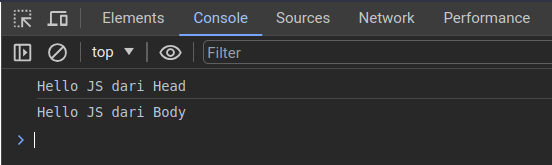
\includegraphics[height=3cm]{./images/p3-n1.png}
    }
    \item {
        It depends on the situation and the needs of the use case.
        If it needs to block the rendering process, then it should be placed in the head tag.
        If it doesn't need to block the rendering process, then it should be placed in the body tag after all the tags.
    }
\end{enumerate}

\subsubsection{Part 2}
\begin{enumerate}
    \item {
        It gives 2 clickable anchor tags that will trigger an \texttt{alert()} function when clicked\\
        
\includegraphics[height=3cm]{./images/p3.2-n1.png}
    }
    \item {
        The first anchor tag is using the \texttt{onclick} property to trigger the \texttt{alert()} function when clicked.
        The second anchor tag is using the \texttt{javascript:} directive on the \texttt{href} property.
    }
\end{enumerate}

\subsubsection{Part 3}
\begin{enumerate}
    \item {
        It prints the text to the console\\
        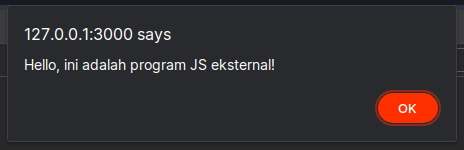
\includegraphics[height=3cm]{./images/p3.3-n1.png}
    }
    \item {
        If the file is moved to a separate directory, then the path should be changed to the new path.
        If we don't do this, then the browser will not be able to find the file and will throw an error.
    }
\end{enumerate}

\subsection{Part 4}

\end{document}

